\section{Liste de capteurs}\label{sec:liste-de-capteurs}

    \begin{figure}[H]
        \begin{center}
            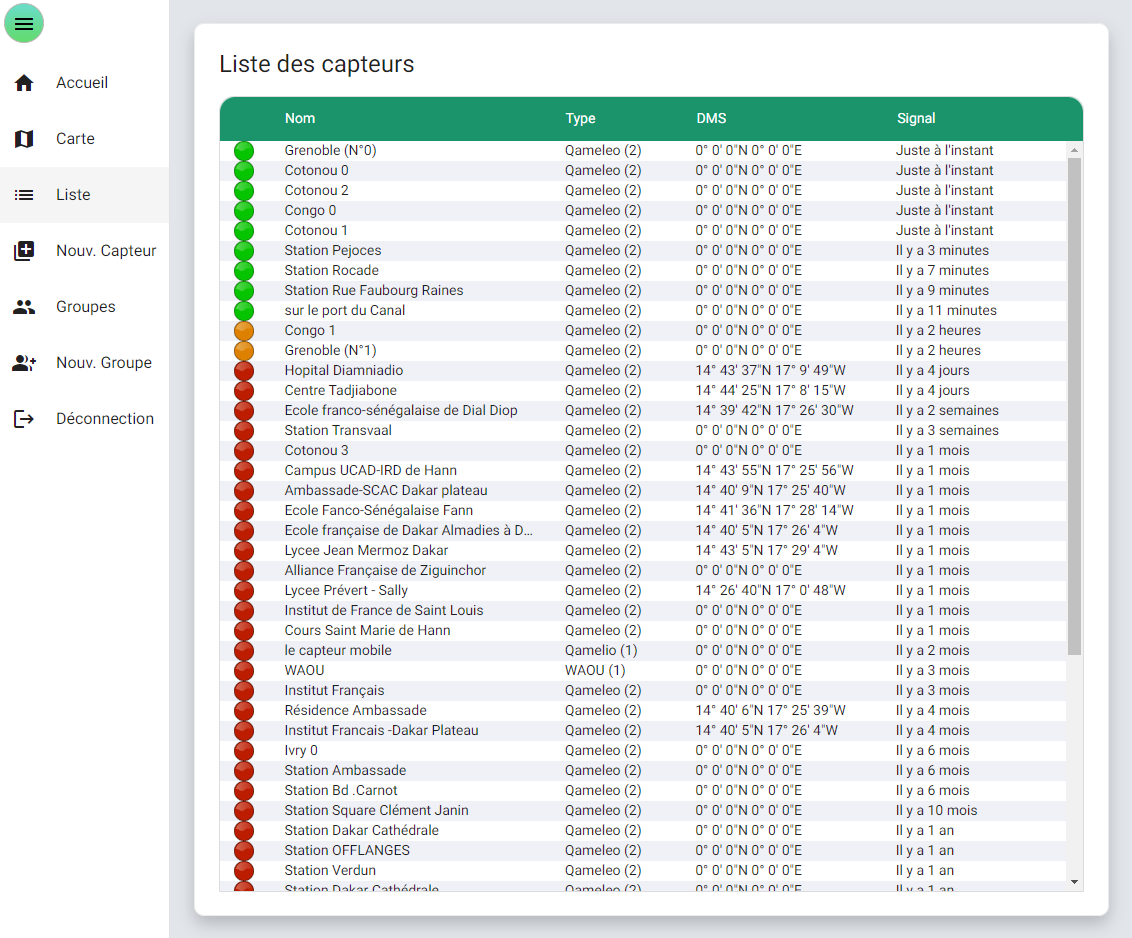
\includegraphics[width=12cm]{resources/list}
        \end{center}
        \caption{Liste de capteurs}\label{fig:liste-de-capteurs}
    \end{figure}

    En cliquant sur ``Liste des capteurs'' depuis la page d'accueil ou ``Liste'' dans le menu à gauche,
    vous pourrez visionner la liste de capteurs à votre disposition.
    Les capteurs sont triés par ordre de dernière émission de données.
    Chaque ligne comporte 5 indications : un voyant indiquant la dernière émission (vert pour moins d'une 1 h,
    orange pour moins de 24h et rouge pour plus d'un jour) puis vous avez le nom du capteur,
    le nom du modèle de capteur, sa position en DMS (degré minute seconde)
    et le temps depuis la dernière réception de données.
    Chaque ligne peut être cliquer pour afficher la page du capteur.
